\section{Interpretabilidade Sináptica e Dinâmica Interativa no Streamlit}
\label{sec:interpretabilidade}

\subsection{Inspeção Visual e Numérica dos Pesos Sinápticos}
As Figuras~\ref{fig:grafo_antes}, \ref{fig:grafo_depois} e \ref{fig:heatmap} apresentam a evolução topológica e numérica dos pesos sinápticos da configuração campeã (\texttt{C4}), atendendo integralmente ao requisito de exibição numérica e espessura proporcional das conexões.

\begin{figure}[H]
    \centering
    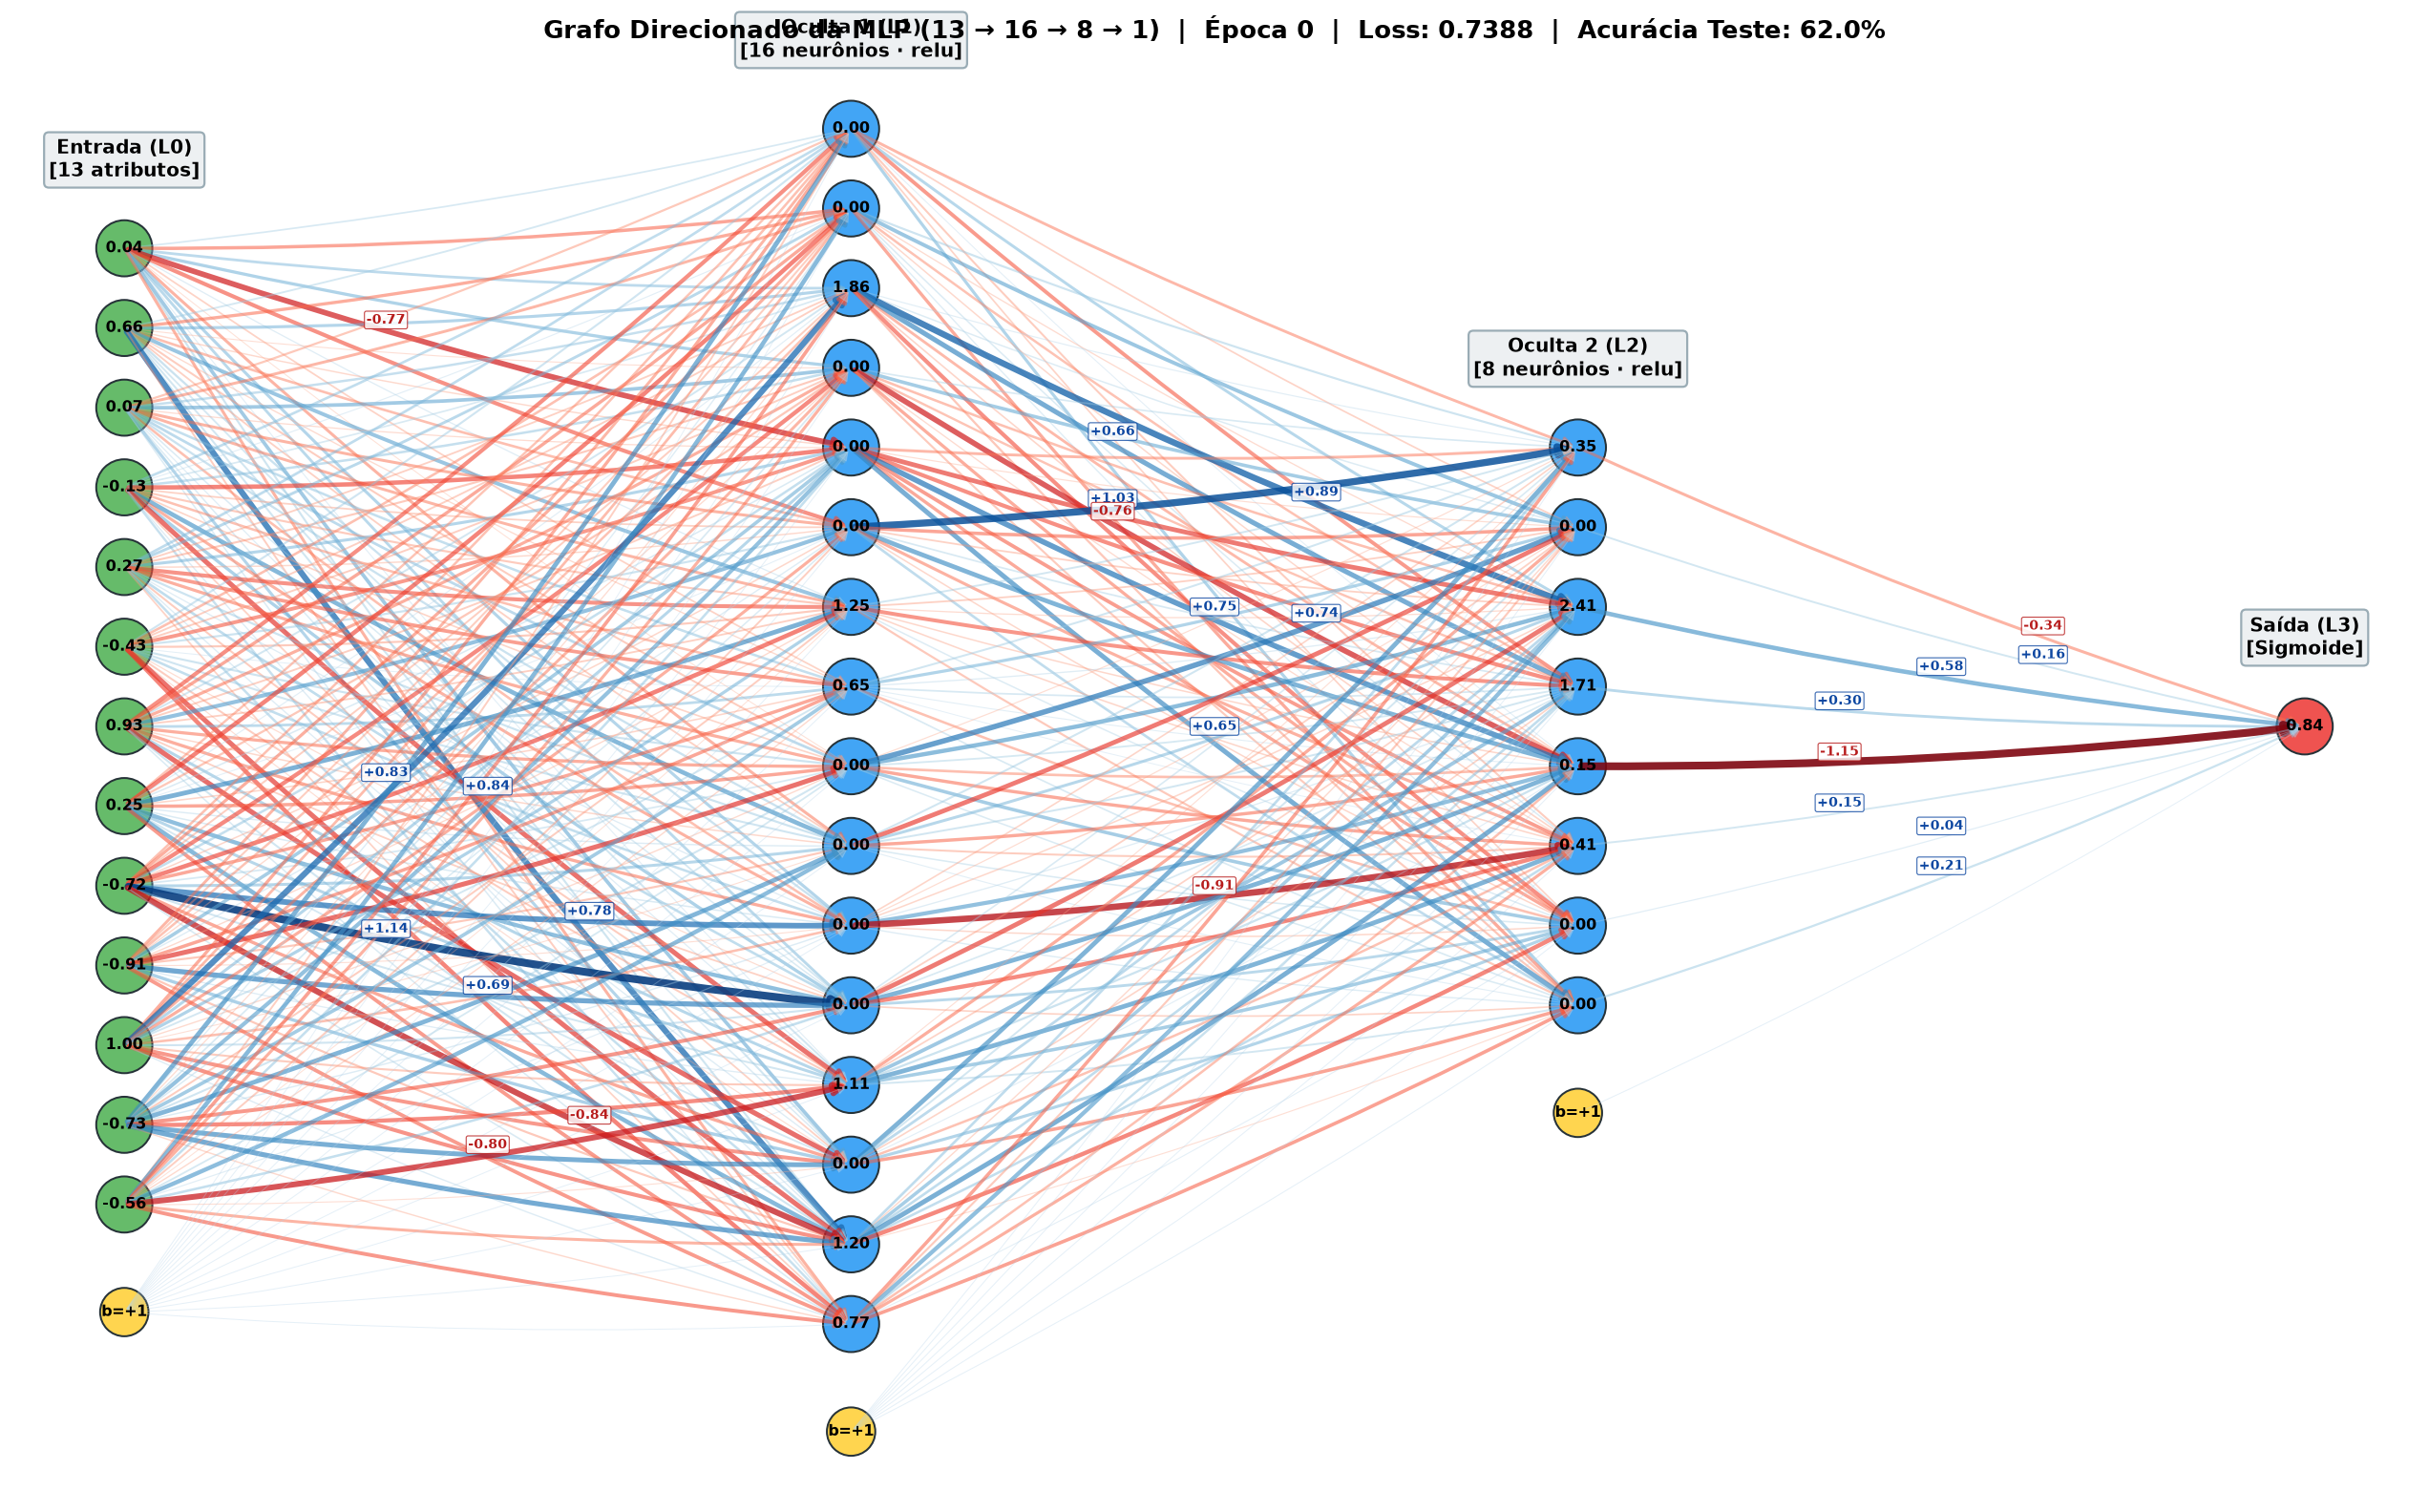
\includegraphics[width=0.92\textwidth]{figs/grafo_antes.png}
    \caption{Grafo direcionado da MLP na Época 0 (antes do treinamento), com exibição numérica dos pesos iniciais e espessura proporcional nas conexões.}
    \label{fig:grafo_antes}
\end{figure}

\begin{figure}[H]
    \centering
    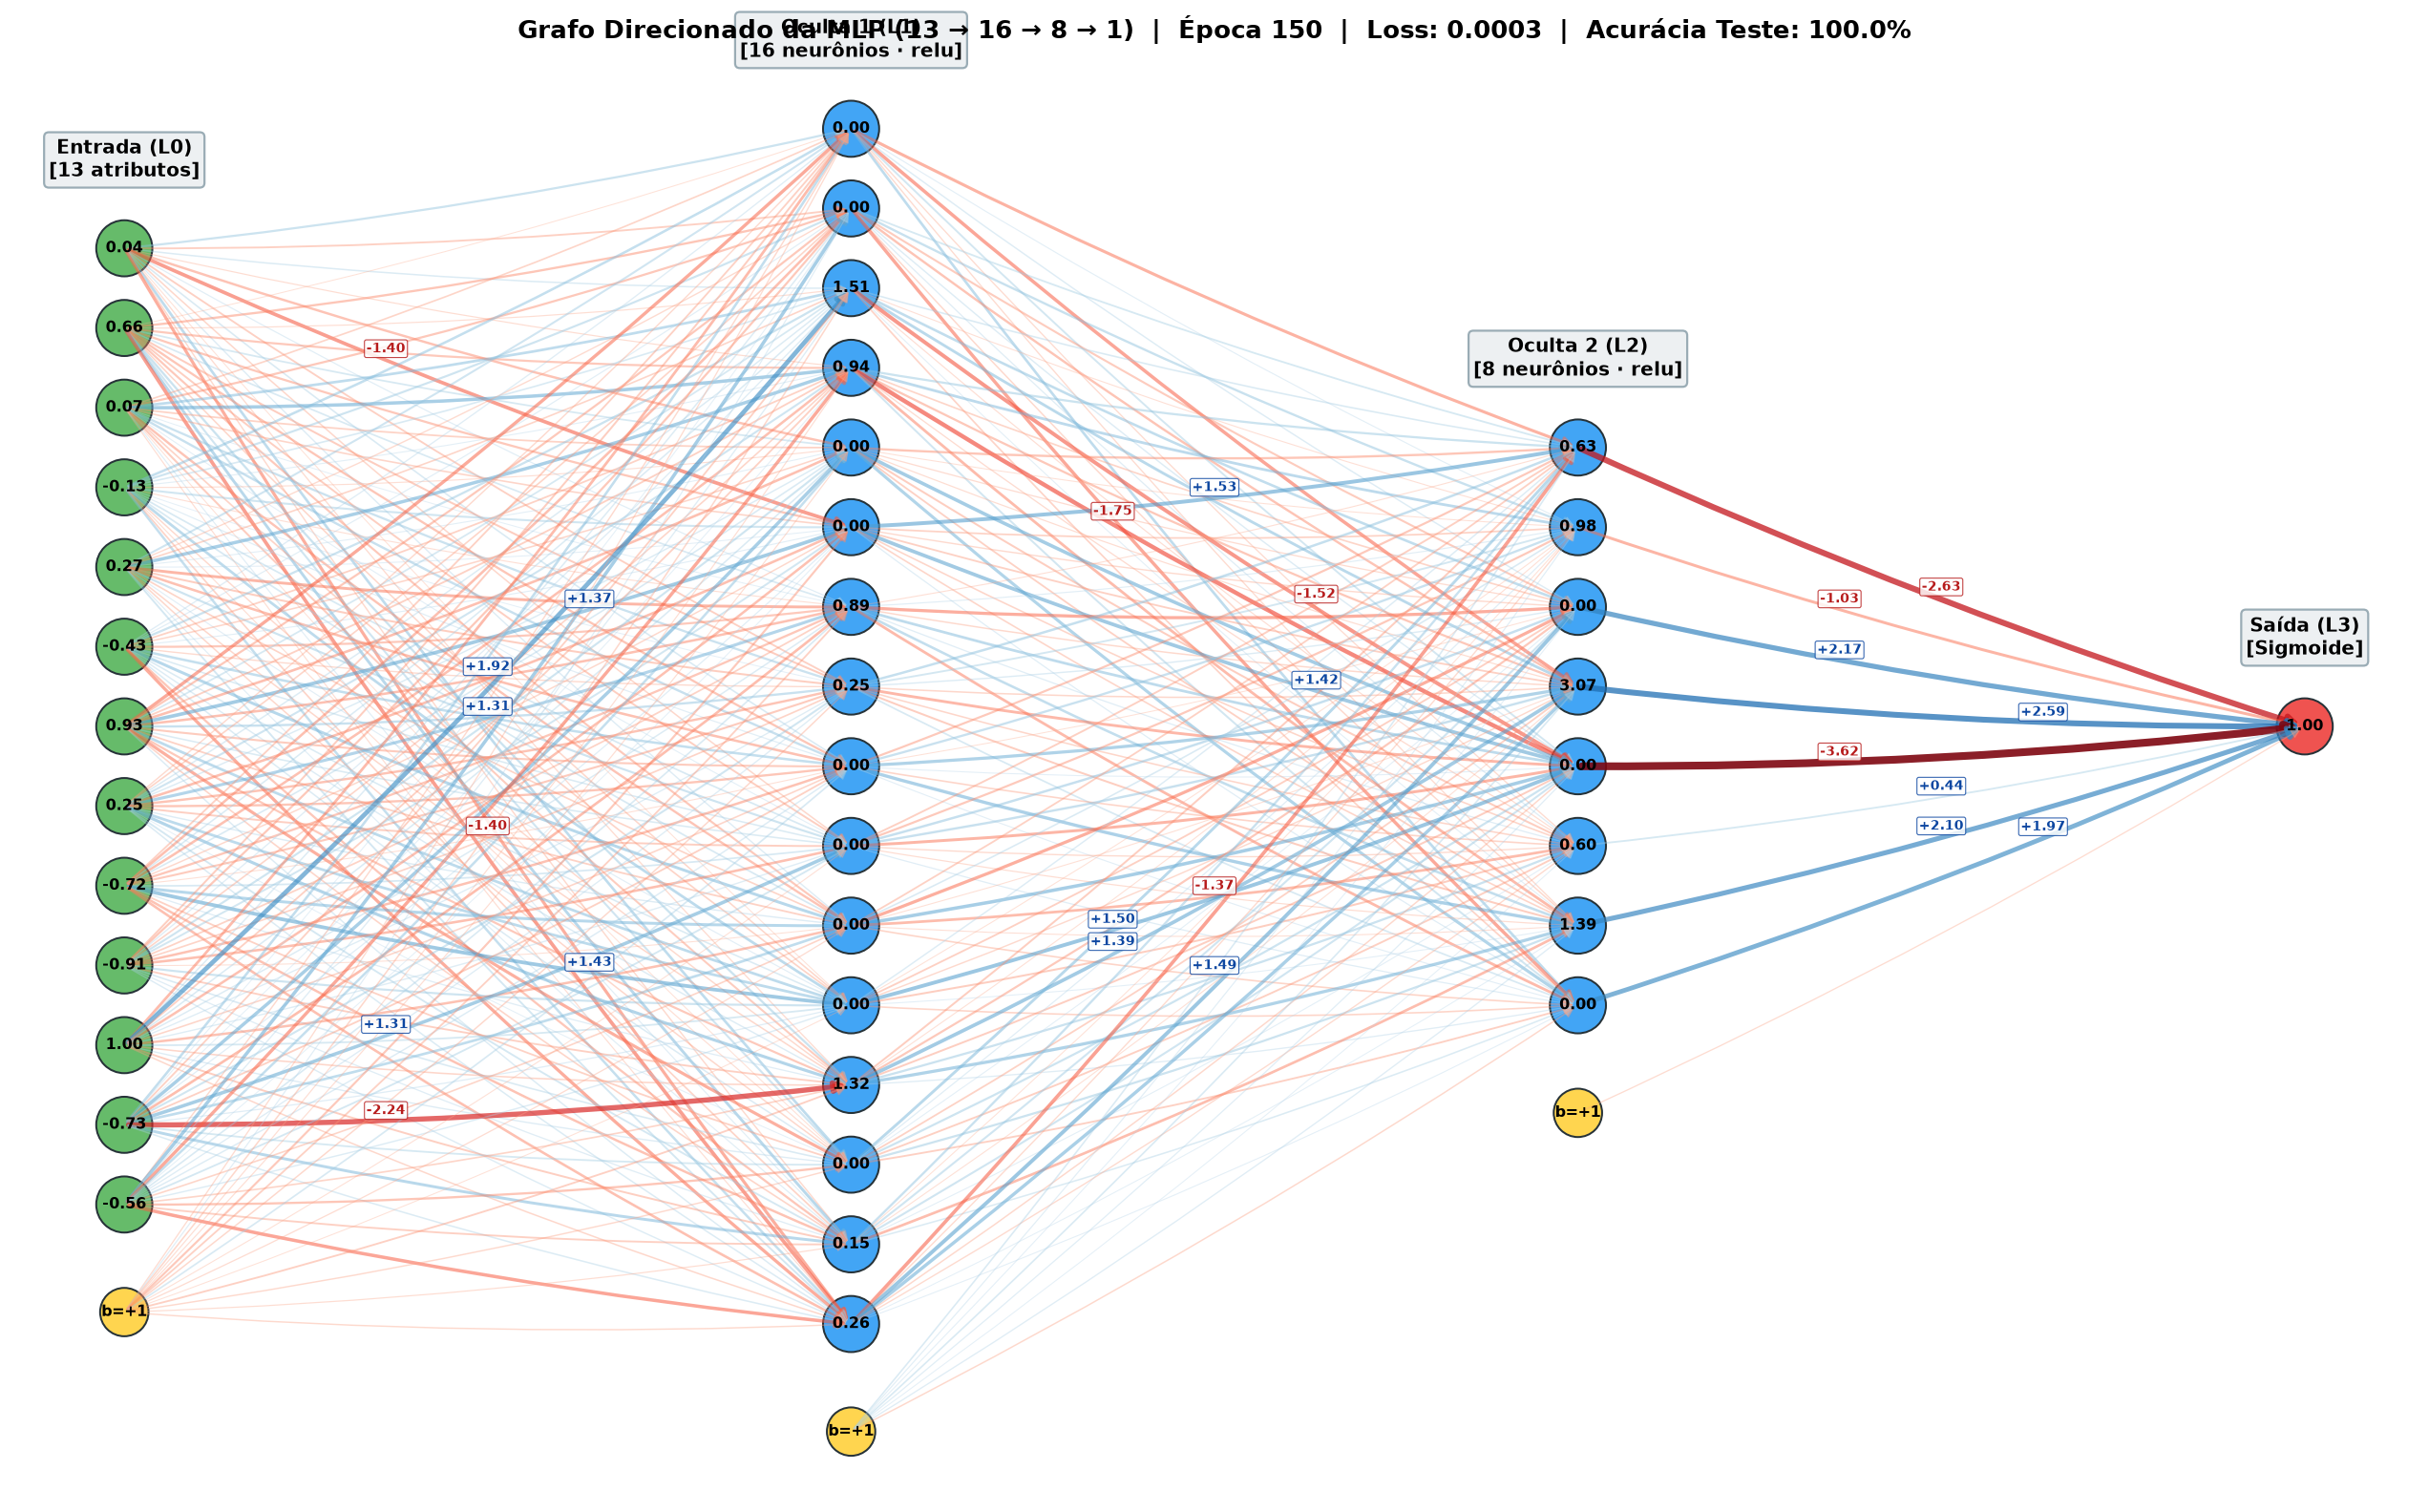
\includegraphics[width=0.92\textwidth]{figs/grafo_depois.png}
    \caption{Grafo direcionado da MLP na Época 150 (após o treinamento da configuração C4), evidenciando o fortalecimento das sinapses discriminativas.}
    \label{fig:grafo_depois}
\end{figure}

\begin{figure}[H]
    \centering
    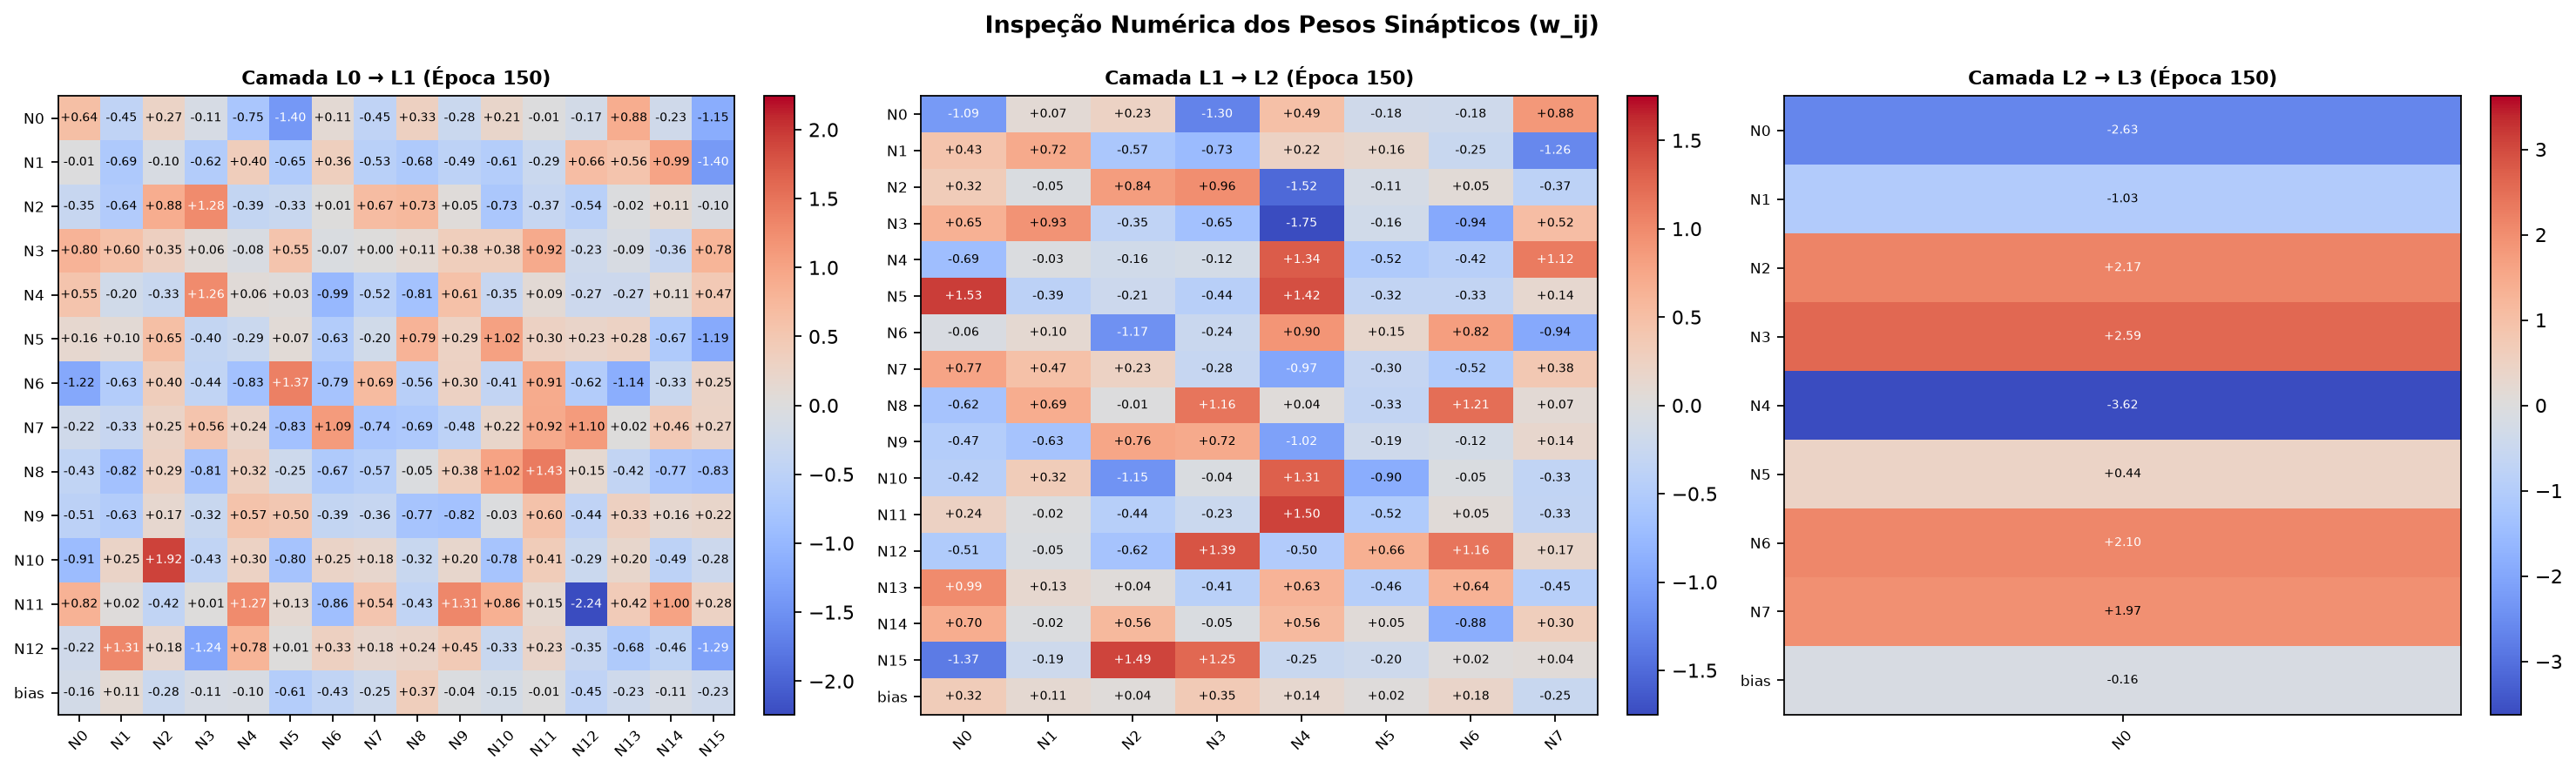
\includegraphics[width=0.98\textwidth]{figs/heatmap_pesos.png}
    \caption{Mapa de calor com anotação numérica explícita dos pesos sinápticos $W^{(l)}$ por camada na Época 150.}
    \label{fig:heatmap}
\end{figure}

\subsection{Interpretabilidade Clínica da Camada de Entrada (\texttt{L0 $\to$ L1})}
Analisando a norma $L_1$ acumulada $\sum_{j=0}^{15} |w_{ij}^{(1)}|$ e os pesos extremos na camada de entrada da rede treinada (\texttt{best\_model\_synaptic\_weights.csv}), verifica-se forte alinhamento com a fisiopatologia coronariana:
\begin{enumerate}
    \item \textbf{\texttt{ca} (\texttt{L0\_N11}, $\sum |w| = 10{,}781$, pico $w = -2{,}2440$ em \texttt{L0\_N11 $\to$ L1\_N12}):} apresentou o maior peso sináptico individual de toda a camada de entrada, refletindo o papel determinante do número de vasos principais obstruídos na fluoroscopia.
    \item \textbf{\texttt{restecg} (\texttt{L0\_N6}, $\sum |w| = 10{,}898$, pico $w = +1{,}3734$):} liderou a soma absoluta de conexões, capturando alterações isquêmicas de onda ST-T no eletrocardiograma de repouso.
    \item \textbf{\texttt{slope} (\texttt{L0\_N10}, pico $w = +1{,}9171$) e \texttt{exang} (\texttt{L0\_N8}, $\sum |w| = 9{,}201$):} destacaram a resposta isquêmica ao teste ergométrico (inclinação do segmento ST e angina de esforço).
    \item \textbf{\texttt{thalach} ($\sum |w| = 8{,}399$) e \texttt{thal} ($\sum |w| = 8{,}283$, pico $w = +1{,}3072$):} quantificaram a reserva cronotrópica e os defeitos perfusionais na cintilografia miocárdica.
\end{enumerate}

\subsection{Dinâmica de Interação em Tempo Real no Streamlit (\texttt{code/mlp/app.py})}
A interface interativa construída em \texttt{Streamlit} integra cinco módulos operacionais: (i) painel lateral de parametrização em tempo real (1 a 4 camadas ocultas, 2 a 32 neurônios por camada, 7 funções de ativação, $\eta$, $\beta$, $\lambda$, decaimento de LR e épocas); (ii) painel de auditoria do particionamento 80/20; (iii) renderização ao vivo do grafo e das curvas de perda e acurácia durante o treinamento; (iv) abas de mapas de calor ($W^{(l)}$ e $\Delta W^{(l)}$) e tabela filtrável de pesos por época; e (v) simulação animada passo a passo do \textit{Forward Pass} (verde neon) e \textit{Backward Pass} (laranja) para pacientes individuais do conjunto de teste.
